%!TEX root = ./intern_report.tex

\subsection{Company Overview}

\paragraph{}
Commonwealth Scientific and Industrial Research Organization (CSIRO) is the Australian federal government agency for scientific research and development.  CSIRO has its headquarters in Canberra, Australia and several branches across the world, with over 5500 employees. CSIRO is known for the development of Wi-Fi, Atomic absorption spectrography and the polymer banknote which have changed the lives of millions of people around the world.

\paragraph{}
CSIRO consists of many parts: Agriculture and Food, Data61, Energy, Land and Water, Mineral Resources...etc with research centers in several cities of Australia. DATA61 is a part of CSIRO that aims on developing a data driven future for Australia. DATA61 consists of multiple groups: robotics and automation group (RAG), data privacy group, mobile security group, distributed sensor networks...etc. 

\paragraph{}
I worked in the Pullenvale (Brisbane) branch of CSIRO. It is called the 'Robotics hub of Australia' due to the large number of robotics projects, facilities and researchers present in the Pullenvale branch. The robotics and automation group of CSIRO is known worldwide for their state-of-the-art SLAM (Simultaneous Locomotion and Mapping) algorithms.

\begin{figure}[h]
\centering

\includegraphics[trim=0cm 0cm 0cm 0cm, clip=true,scale=1]{figures/data61_logo.png}
\caption{DATA61 logo\label{Fig:data61}}\vspace{-4mm}
\end{figure}


\subsection{Company History}

It was formed in 2015 by merging NICTA (National Information and Communications Technology Australia Ltd) with CSIRO's data science section. 

\subsection{Organization Structure and Hierarchy}
\subsection{Areas of Interest}
\subsection{Current Situation}

\paragraph{}
The RAG of CSIRO was recently selected as one of the six teams worldwide for the DARPA Subterranean Challenge by United States Department of Defense. Therefore the next four years of research in Robotics in CSIRO will be more focused on developing robots that can simultaneously map and navigate underground tunnels, caves and mines without GPS or reliable communication with humans. For this task, incorporating machine learning into the workflow of algorithm development and testing is of paramount importance for all researches in RAG. I addressed this problem by developing an efficient end-to-end pipeline for this and demonstrating it through two projects.

\subsection{Impacts on Sri Lankan Industry}

\subsection{SWOT Analysis}
\subsubsection{Strengths}
\subsubsection{Weaknesses}
\subsubsection{Opportunities}
\subsubsection{Threats}

\subsection{DARPA Subterranean Challenge}
\label{ssec:darpa}

%Image: Darpa challenge
\begin{figure}[H]
    \centering
    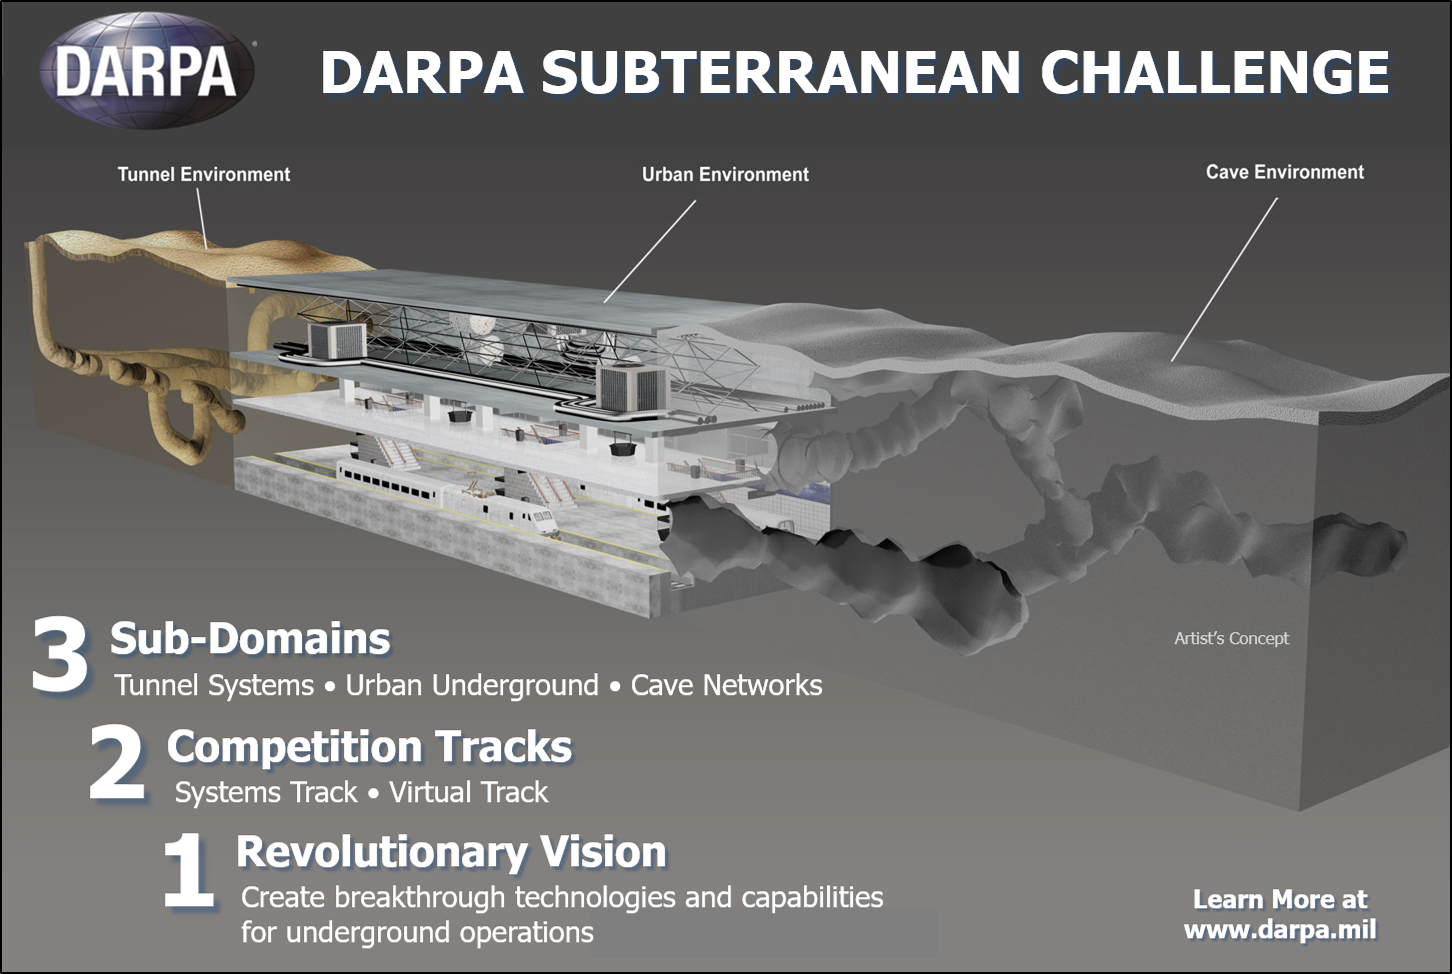
\includegraphics
        [width=15cm]
        {figures/subt_challenge.png}
    \caption{CSIRO focuses on DARPA challenge}\vspace{-4mm}
\end{figure}

\subsection{Usefulness to the Country}
\subsection{Suggestions to Improve the Company}